\section{LabVIEW Symbolic Systems Tutorial}  


When you write down a transfer function, you probably want to write it down in
terms of of the inertial, damping, and spring parameters.  That is, you want to
write down the \emph{symbolic} transfer function--the transfer function that has
not yet been evaluated for a particular choice of parameter values.  It would be
nice to be able to write the transfer function in LabVIEW in a similar way to
allow easy changes in the transfer function as you alter values of your
parameters.  Fortunately, LabVIEW has a way of doing this.

\begin{center} \textbf{Steps for Creating a Symbolic Transfer Function}
\end{center}
To create a symbolic transfer function, one must use the transfer functions from
the Control Design Toolkit.  The steps for doing this are as follows.
\begin{enumerate}
\item Make a Simulation environment from the Simulation Module Palette.
\item Go to the Control Design Palette and get a Transfer Function from the
  Model Construction Sub-Palette.  
\item On this transfer function, select \emph{Single-Input, Single-Output (Symbolic)}.
\item On the top left of the transfer function block there is an input to the
  block that is the ``Symbolic Numerator'' and an input that is the ``Symbolic
  Denominator.''  Moreover, on the bottom of the block there is an input called
  ``Variables.''  For each of these inputs you should right-click, go to
  \emph{Create}, and select \emph{Constant}.  You should now have three arrays
  with arrows going into your transfer function block.
\item Drag these three sets of blocks away from each other so that you have some
  room to work with.  Expand the right-hand side of each of these arrays into a
  column vector by dragging the bottom right corner of the right hand block
  down.
\item Now you may put symbols into the numerator and denomenator so long as you
  define the value of those symbols in the ``Variables'' block.
\item In order to use this transfer function in the Simulation Module, you will
  need to use a conversion block in the Control Design Palette from the Model
  Conversion Sub-Palette.  Use the block called
  ``CD~Convert~Control~Design~to~Simulation.vi.''  Select \emph{SISO TF} on this
  block.  
\item Now connect the output of your transfer function to the input of this
  block and connect the output of this block to your simulation transfer
  function.  You will need to select Terminal for Parameter Source in your
  transfer function block so that you can connect to it.  
\item A completed loop would look something like what is found in
  Fig.\ref{fig-symboliclabview} (with a proportional controller).
\begin{figure}[t!]
\centering
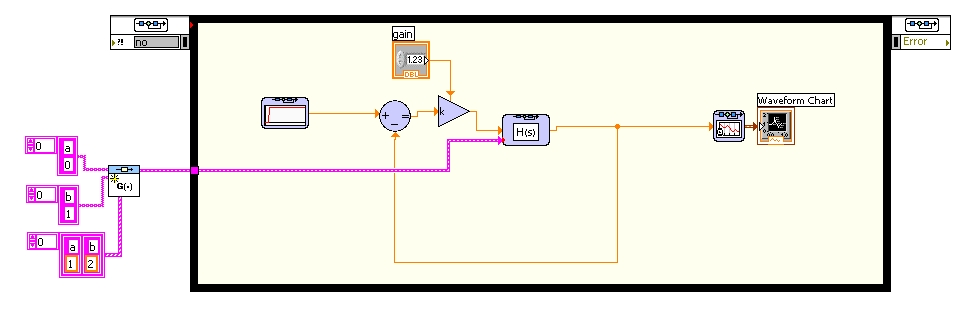
\includegraphics[width=6in]{symbolic/SymbolicTF}
\caption{A LabVIEW program with a symbolic transfer function $\frac{RL}{Ls+R}$,
  where $R=10$ and $L=2$.}
\label{fig-symboliclabview}
\end{figure}
\item More details can be found in the Control Design Toolkit Manual, which is
  available online from National Instruments at ni.com.  A Google search should
  find it for you reasonably quickly.  
\end{enumerate}
\newpage
\begin{center} \textbf{Steps for Creating a Symbolic State Space Model}
\end{center}


\begin{figure}[t!]
\centering
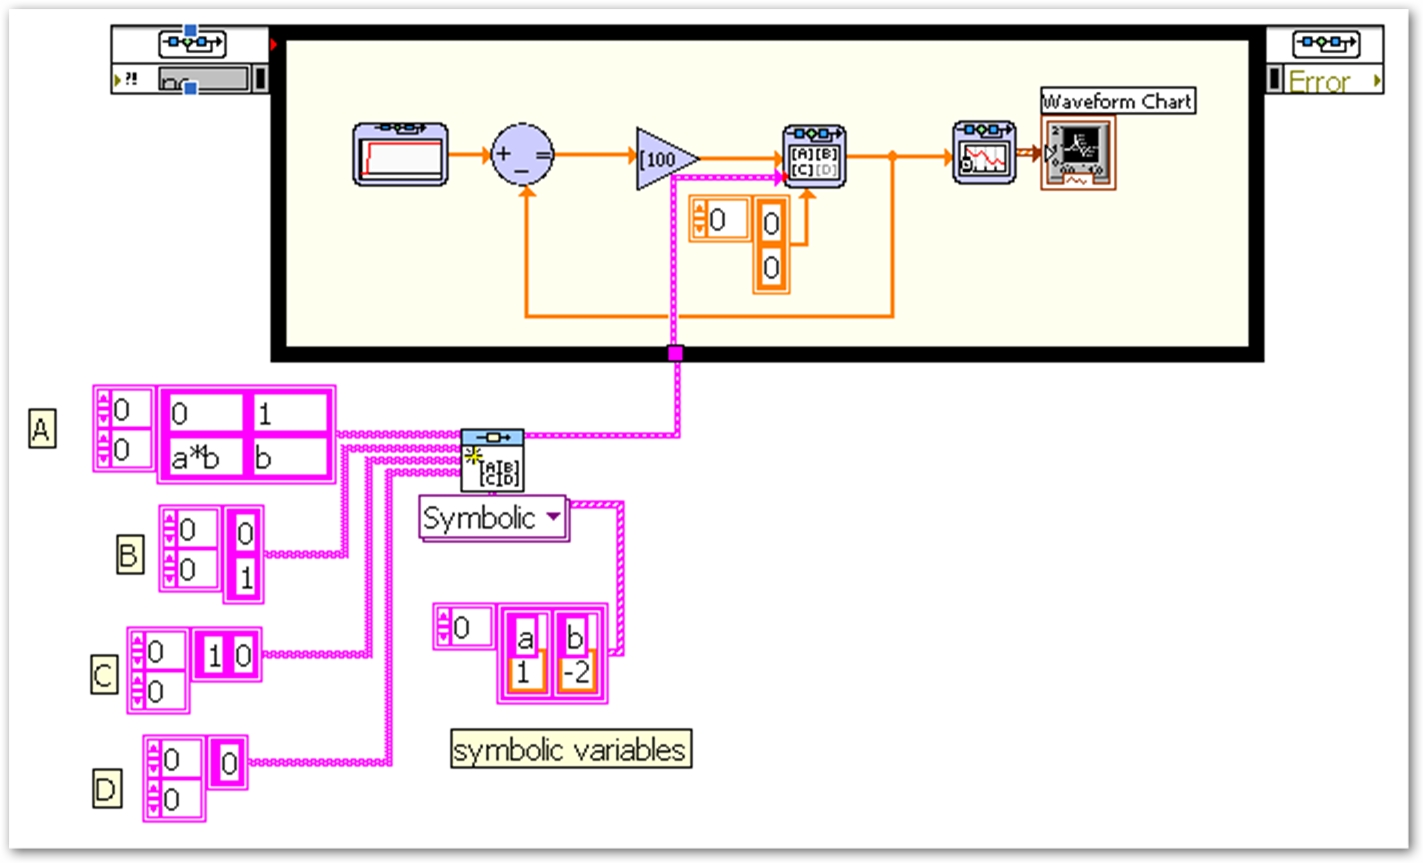
\includegraphics[width=6in]{symbolic/symbolicSS}
\caption{A LabVIEW program with a symbolic state space system}
\label{fig-symbolicSS}
\end{figure}


Symbolic State-Space Systems are roughly the same procedure.
Fig.~\ref{fig-symbolicSS} shows a symbolic state space system with
$A=\left[\begin{array}{cc} 0 & 1 \\ RL & L \end{array}\right]$,
$B=\left[\begin{array}{c} 0 \\ 1 \end{array}\right]$, $C=\left[\begin{array}{cc}
    1 & 0 \end{array}\right]$, $D=0$, where $R=1$ and $L=-10$.  The main thing
you need to be careful of here is that you must put a ``Build Array'' block
(from the ``Array'' Pallette)
after the reference input.  Also, note that you \emph{must} specify the initial
conditions of your system in the state space block from the simulation module.
Keep in mind that these must be of the same dimension of your system, so for a
six state system you must have six initial conditions.
 

%% Local Variables:
%% TeX-master: "../LVmanual.tex"
%% End:

